\section{Anaxia: the engine}\label{sec:network}

The theorems of the preceding sections price the checking of candidates and bound the number of proposals any proposer needs. They say nothing about where candidates come from. This section describes Anaxia, the engine we built to supply them, in the order in which a candidate meets its parts. In the crossing network, known constructions are typed nodes, new candidates are crosses of old ones, every cross is checked and then refuted if possible, and every outcome is written to a memory that steers the next cross (Fig.~\ref{fig:channel}). Construction mode writes down a new object, a graph, together with the argument for what it forces, and has it checked again by code that shares nothing with the search. The tower of Section~\ref{sec:towers} stacks construction mode into layers. A registry records what each part takes from earlier systems, and the whole is released as one package.

\begin{figure*}[t]
\centering
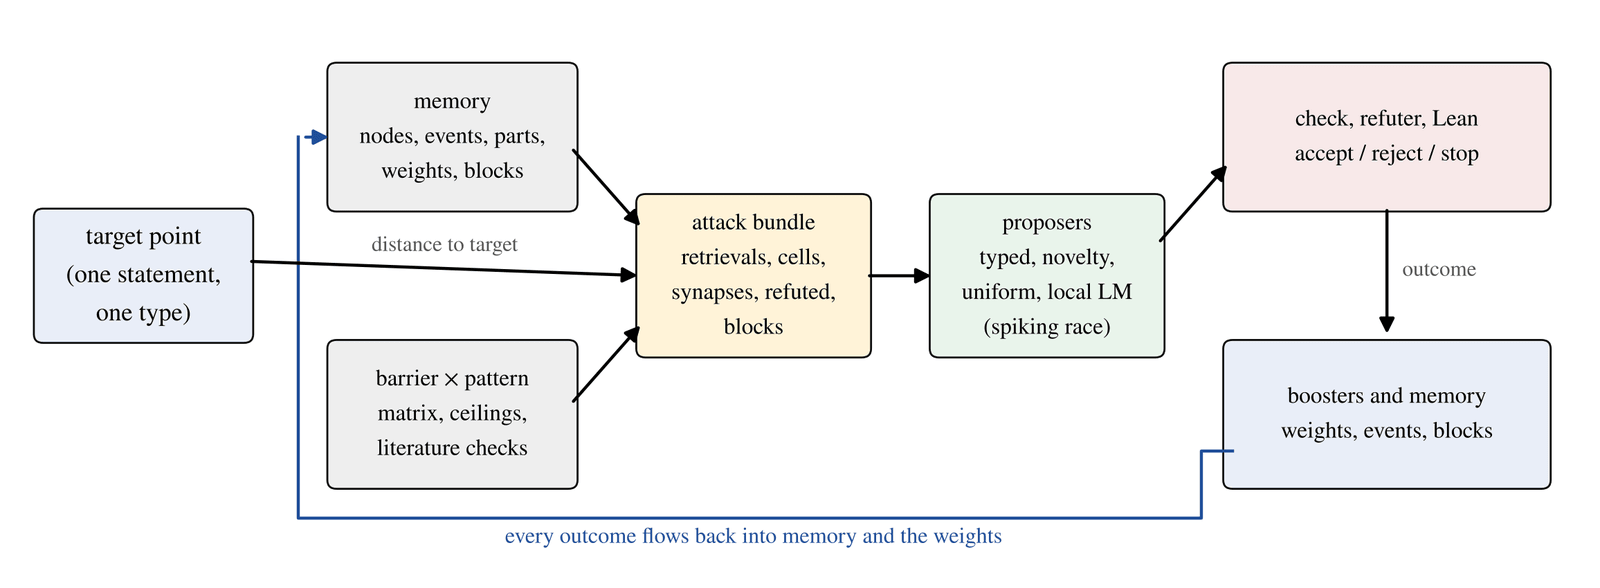
\includegraphics[width=0.98\textwidth]{figures/fig_channel}
\Description{Diagram of one round of the attack loop: a target type, the distance of each composite to it, and the attack bundle fed back to the generator.}
\caption{One round of the attack loop. The target point of a benchmark fixes a type; every composite gets a distance to that type. The attack bundle collects, for each candidate cross, the most similar past attempts in memory, the cells of the barrier and pattern matrix that touch its parts, the weights of its synapses, the refuted offspring of its parts and the blocks recorded on its problem. The proposers draw from the weighted candidates; the check, the refuter and, for a new statement, Lean decide the outcome, which updates the boosters and the memory before the next round.}
\label{fig:channel}
\end{figure*}

\subsection{Constructions as typed nodes}

A \emph{construction} $c$ is a record of three items: $\mathrm{gives}(c)$, the type of the object it produces; $\mathrm{needs}(c)$, the list of types it consumes; and $\mathrm{source}(c)$, the published result or computation it comes from. The single-link law of $\mathrm{SU}(2)$ gives a link law and needs nothing; Dobrushin's uniqueness criterion \cite{Dob68} gives a range of couplings and needs a dependency graph and an influence bound; Shioda's inductive structure \cite{Shi79} gives a splitting of a Fermat character and needs a character table. If $\mathrm{gives}(b)\in\mathrm{needs}(a)$, the \emph{cross} $a\leftarrow b$ is the construction with the first such input of $a$ filled by $b$; its parts are the union of the parts of $a$ and $b$. A composite with no unfilled input is \emph{closed}, and only closed composites are checked. Typing removes ill-formed candidates before any check: on the Yang--Mills library, crossing without regard to types wastes $45.4$ of $48$ crosses per run on ill-typed pairs (Table~\ref{tab:boosters}).

The library of a benchmark is the set of its constructions. Five libraries are used: Yang--Mills ($38$ nodes), Hodge ($28$), the standard conjecture of Lefschetz type ($17$), Chowla's conjecture ($20$) and Erd\H{o}s problem 1183 ($13$). Of these $116$ nodes, $54$ are literature constructions written out with their key lemma and the barrier at which they stop, for instance the Kotecký--Preiss criterion, the Brydges--Yau and Gaw\c{e}dzki--Kupiainen block-spin flows, Holley--Stroock and Stroock--Zegarlinski for Yang--Mills; van Geemen, Ribet, Kuga--Satake, Varesco and Charles--Markman for Hodge; Friedlander--Iwaniec, Heath-Brown, Green--Tao and Matomäki--Radziwi{\l}{\l}--Tao for Chowla.\footnote{The list is the file \texttt{knowledge.json} of the package. Each entry carries the problem it addresses, its typed inputs and output, the published source, the lemma that does the work, and a verdict: \emph{known} when the construction proves a published statement, \emph{stops} when it is known to fail at the benchmark's blocking step, with the reason. A literature node is never counted as progress: a composite that reaches a known statement is accepted as known and rewarded at a quarter of the rate of a new one, and a composite through a node marked \emph{stops} is stopped with that node's reason.}

\subsection{Checks and the refuter}

The check of a closed composite is a program attached to its output type. It returns \emph{accepted} with a measurement, \emph{rejected} with the measurement that failed, or \emph{stopped} when no checkable form of the composite exists. On Yang--Mills the check of a Dobrushin composite counts the active partners of a link in the dependency graph the composite names and computes the range $\beta_{W}<1/(\text{partners}\cdot\frac14)$ from the influence bound; on the Fermat fourfolds it enumerates the zero-sum splittings of the characters in an orbit; on Erd\H{o}s problem 1183 it computes the largest monochromatic sublattice by the search of Lemma~\ref{lem:levelposet}. An accepted composite then meets the \emph{refuter}, which breaks it if its range is dominated by one already known, if it reproduces an accepted statement without gain, or if it rests on an unrefereed claim. Only composites that pass both count as survivors. A survivor whose statement is new is formalised in Lean before it is reported; none of the five pass lines has such a survivor.

\subsection{Boosters}

Every ordered pair of library heads carries a synapse with weight $w$, initially $1$. When a cross fires and its offspring survives, its synapse rises by $\eta$, and the synapses that built its parents rise by $\eta\gamma^{k}$ at distance $k\le4$; a rejected or refuted offspring lowers its synapse by $\eta/2$, to no less than $0.05$. After each generation the weights leaving each node are rescaled to mean one, and a share $\eps$ of the crosses is drawn uniformly. We use $\eta=1$, $\gamma=\frac12$ and $\eps=0.2$. This is a Hebbian rule with path credit, and Section~\ref{ssec:boosters} measures what it adds.

\subsection{Memory}

The memory is one SQLite store shared by every proposer and every round. It holds the nodes, one event per checked composite (its parts, outcome, measurement, reason, synapse weight, round and proposer), an index from parts to events, the synapse weights, the blocks (for each problem and step, the assumption that stopped it and the source of the stopping composite), the literature checks, and a log of every retrieval. Two uses follow.
\begin{enumerate}[label=(\roman*),leftmargin=1.8em,itemsep=1pt]
\item \emph{Decided composites are skipped.} A composite whose parts already have an event is not checked again; this is what removes the repeated checks of Fig.~\ref{fig:memory}(b).
\item \emph{Retrieval steers the draw.} For a candidate with part set $Q$, the $k=5$ past events with the largest score $J(Q,S)\,w$ are retrieved, where $S$ is the part set of the event, $J$ the Jaccard similarity and $w$ the synapse weight at the time. The candidate's weight is multiplied by
\begin{equation}\label{eq:memprior}
\pi_{\mathrm{mem}}(Q)=\min\Bigl(3,\ \max\Bigl(\tfrac14,\ 1+\sum_{\text{survivors}}J-\tfrac12\sum_{\text{others}}J\Bigr)\Bigr),
\end{equation}
which raises it near past survivors and lowers it near failures.
\end{enumerate}
The store of a five-round study over all five libraries holds $42$ events, $11$ blocks and $26$ weights in $156$ kilobytes, so the memory is small and the check, not the bookkeeping, is the cost.

\subsection{Target points and the attack channel}

A \emph{target point} is one statement whose proof would cross the wall of a benchmark, together with its type. For Erd\H{o}s problem 1183 it is a family of colourings of $2^{[n]}$ whose monochromatic sublattices have at most $n/2+C$ members for every $n$; for Yang--Mills, an effective action at one coupling $\beta_{W}>\frac13$ whose blocked measure satisfies a Dobrushin-type condition uniformly in the spacing; for Hodge, the algebraicity of the class of the character $(1,16,26,31,36)$ of level $55$ on the Fermat fourfold of degree $110$; for Chowla, local $U^{2}$ uniformity of the Liouville function on almost all intervals of length $\exp((\log X)^{2/5-\delta})$, one step below the scale of \cite{Pil26}; for the standard conjecture, an algebraic inverse of $L$ on $H^{2}$ of one threefold of general type with $h^{2,0}>0$. A backward search over the library gives every type a distance: $0$ for the target type, and $1+d$ for each input of a construction whose output is at distance $d$. A candidate's weight is multiplied by $e^{-d}$, where $d$ is the distance of its output, so the forward search by crossing and the backward search from the target meet at the composites of distance $0$ and $1$.

The \emph{attack channel} is the single pipeline that hands everything the engine holds to the proposers. For each candidate it builds a bundle: the retrievals, the cells of the barrier and pattern matrix that touch its parts (Section~\ref{ssec:matrix}), the weights of its synapses, the refuted offspring among the retrievals, and the blocks of its problem. The bundle multiplies the weight by
\begin{equation}\label{eq:channelprior}
\pi_{\mathrm{ch}}=\min\Bigl(5,\ \max\Bigl(0.05,\ 2^{-n_{\mathrm{fail}}}\,(\tfrac32)^{n_{\mathrm{part}}}\bigl(1+\textstyle\sum_{\text{survivors}}J\bigr)\Bigr)\Bigr),
\end{equation}
where $n_{\mathrm{fail}}$ and $n_{\mathrm{part}}$ count the cells of the bundle whose recorded outcome is a failure or a partial result. Every bundle that flows is written to the memory, so that a run with the channel can be compared with one without.

\subsection{Proposers and agents}

Four proposers share the weighted candidates: \emph{typed} draws in proportion to the weight; \emph{novelty} takes the candidate least similar to anything in memory; \emph{uniform} draws uniformly; and \emph{local model} shows the eight heaviest candidates and the retrieved notes to a local language model with $5\times10^{8}$ parameters \cite{Qwe24} and takes the one it names. Which proposer moves is decided by the spiking selector of Proposition~\ref{prop:spiking}, rewarded on survivors, so that the committee samples the square root of each proposer's record of success, the optimum of Theorem~\ref{thm:I}.

An \emph{agent} holds one target point, its own library, its own synapse weights and its slice of the shared memory. Each step it attacks its library through the channel. When a step adds no survivor it runs a sub-attack whose target is the nearest open input type of its target point, a lemma at distance one. Agents trade through the memory: a result passes from one agent to another only where one benchmark is an input of another, which among the five happens once, since the standard conjecture for $X$ is a case of the Hodge conjecture on $X\times X$. Both are package code, not language-model agents: an agent is an object with a library, weights and a memory slice, and its step is a call of the attack.

\subsection{Construction mode}\label{ssec:construct}

The crossing network only combines results that someone has already proved. Construction mode builds an object that no one has written down, on problems where the object is finite: planar graphs whose proper $3$-colourings are constrained at a few \emph{contact} vertices on one face. Such a graph is a \emph{gadget}; it is a not-all-equal forcer if no proper $3$-colouring gives its three contacts one colour, and its \emph{profile} is the list of distances between its contacts. Gadgets of this kind are the building blocks of the refutation of Steinberg's conjecture by Cohen-Addad, Hebdige, Kr\'al', Li and Salgado, a planar graph with no cycles of length $4$ or $5$ that is not $3$-colourable \cite{CHK17}, and of every attempt on Erd\H{o}s's question whether a planar graph with no cycles of length $4$, $5$ or $6$ is $3$-colourable.

The builder grows a gadget together with its forcing argument. It assumes that the contacts share a colour $\gamma$ and applies four moves: \emph{attach} a new vertex next to a $\gamma$ vertex, which is then not $\gamma$; \emph{link} two vertices that are not $\gamma$, whose colours then differ; \emph{derive} a new vertex next to two vertices whose colours are known to differ, which is then $\gamma$; and \emph{close} with an edge or a triangle that leaves no colouring. A library gadget may also be inserted as a lemma, with its contacts sent to vertices of the graph. Between moves the builder propagates the forced colours to a fixed point and adds structure only when nothing more follows. Every move passes a cascade of tests before it is kept: no cycle of a forbidden length through a new edge, contact distances at least those of the profile, and planarity with the contacts on one face; only then does an exact satisfiability check decide whether the contacts can still share a colour. When they cannot, the graph is minimised and offered to the gate.

The \emph{gate} is code that shares nothing with the builder: planarity by the left--right algorithm of \texttt{networkx}, every cycle of forbidden length by depth-first search, the contact distances by breadth-first search, and the absence of a colouring with equal contacts by plain backtracking with no satisfiability solver. A gadget counts only when the gate accepts it, and the whole counterexample assembled from a gadget is checked again by three satisfiability solvers, CaDiCaL, Glucose and MiniSat. A second search writes the forcing condition as an exists-forall problem: a satisfiability instance over the edge variables, with planarity built in by a $2$-page book embedding and every $3$-colouring that defeats a candidate turned into a clause that every forcer satisfies. The cost of every run is counted in exact satisfiability checks, so that different searches can be compared at the same budget.

\subsection{The tower of builders}\label{ssec:tower}

The tower $B^{n}$ of Section~\ref{sec:towers} is built over construction mode. Layer~$1$ is the builder with one fixed strategy: the order in which it tries the four moves, how much noise it adds to that order, and how often it tries a lemma. Layer~$2$ acts on layer~$1$: it keeps a population of strategies, runs each for a slice of checks, keeps the better half by gadgets found per check and refills the population with mutations of the survivors, the evolve-and-evaluate loop of FunSearch and AlphaEvolve \cite{RBN24,NVE25} with a fixed space of strategies in place of program text. It also sets a curriculum, as AlphaProof trains on variants of a target before the target \cite{HMS25}: a weaker contact profile is attacked first, and the gadget it yields joins the library as a lemma for the harder one. Layer $k\ge3$ acts on layer $k-1$ by successive halving \cite{JT16}: it runs several copies of layer $k-1$ with different settings and keeps the better half after each round.

Two wirings are compared. In the \emph{ladder} each copy of a layer has its own library and sees only what the layer directly below returns. In the \emph{mesh} every layer reads and writes one library, so a gadget found at the bottom of one branch is a lemma everywhere at once, and the move kinds carry Hebbian synapses \cite{Heb49}: the moves that built a gadget the gate accepted are strengthened by $\eta=1$ shared among them, every synapse decays by a factor $0.95$ at each success, and a strategy's priority for a move is lowered by $1.5$ times its synapse, so that moves that have worked are tried earlier by every layer. Whatever path a gadget took, it counts only after the gate, and the budget of a run is the number of exact checks it spends.

\subsection{What the engine takes from other systems}\label{ssec:sources}

Every system, corpus and method that Anaxia draws on is a record of one registry: its reference, its status (refereed, preprint, software or unrefereed claim), what was taken, the module that implements it, what Anaxia adds and what was left out. The registry has $35$ entries in eight groups, Google DeepMind, methods, OpenAI, The Omega Institute, memory, agents, corpora, and provers and models; Appendix~\ref{app:sources} lists them. Three corpora are indexed as literature and searched before a target is attacked, to see whether it is already settled: the $5{,}035$ items of the public repositories of Google DeepMind, among them $1{,}471$ open and $2{,}437$ solved statements of Formal Conjectures; the $782$ problem dossiers of OpenRefute, each a published conjecture with a Lean claim and a kernel-checked resolution \cite{OIT26}; and the $722$ manuscripts of OpenAI's collection \cite{OAI26b}, every one marked unrefereed. Nothing in an index is used as a lemma by a check, and nothing fetched is executed. No model weights are bundled with the engine.

\subsection{The package}\label{ssec:package}

Anaxia is released as the Python package \texttt{eBLLM}, with the command \texttt{anaxia}, a Lean~4 library and the container image \texttt{ghcr.io/creelie/bllm-engine}, which tells a running copy when a newer image is published; the package is archived under \anaxiaDOIlink \cite{Bha26c}. Its core implements the verifier-gated engine of \cite{Bha26a}. It contains no source code of any language model; hosted models are called through their public interfaces with the user's key and local models through \texttt{llama.cpp}. Its parts are the schedules of Sections~\ref{sec:entropy} to~\ref{sec:towers}; the proposers; the libraries and the literature constructions; the checks, which are the Lean kernel, exact evaluation, randomized polynomial identity tests \cite{Sch80,Zip79}, the searches of Lemma~\ref{lem:levelposet} and of its grid version in C, the gate of construction mode and arbitrary commands with checked output; the memory, the boosters, the channel and the agents of this section, with every kept result also written as a Markdown note linked to the results it uses, so that the memory can be opened as an Obsidian vault and searched with the neighbours of each hit; construction mode, with its gadgets and its reflexive polytopes, and the tower; the learn-from-failure loop with its rule book, its log and its screens; the registry and the three indexes; the six benchmarks with their pass lines; and a Lean development whose finite parts back the theorems of the paper. One command runs the tests, the memory study and the agent loop, and the hardware each part needs is measured in Appendix~\ref{app:hardware}.
